\documentclass{standalone}
\usepackage{tikz}
\usepackage{xcolor}
\usetikzlibrary{patterns, positioning}
\usetikzlibrary{shapes.misc}
\usepackage[outline]{contour}
\contourlength{1.5pt} 


\begin{document}
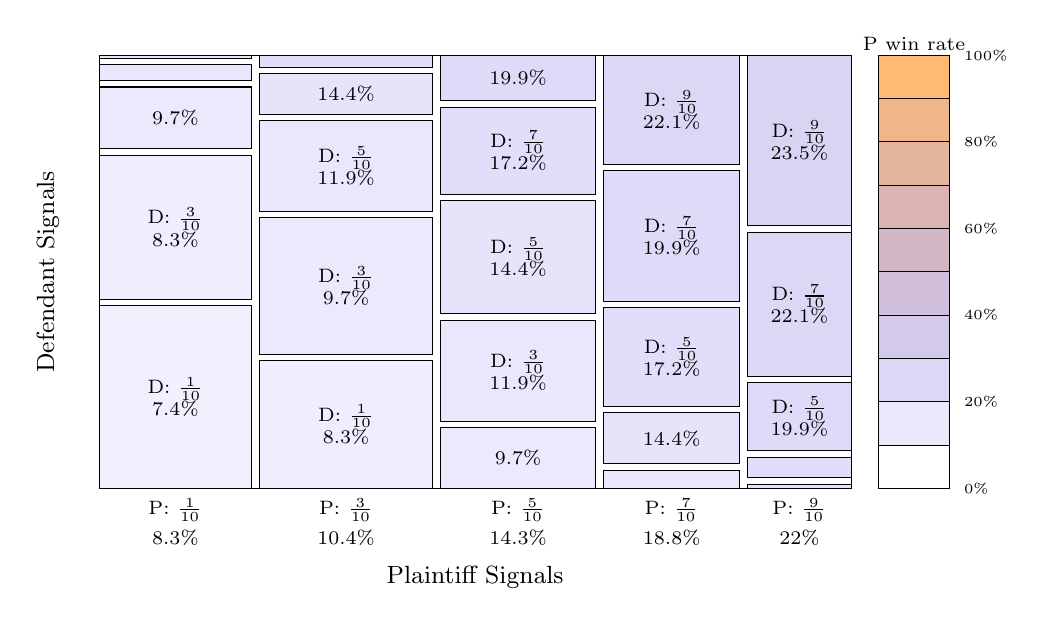
\begin{tikzpicture}
\newcommand{\DFractionOffset}{0.4}
\newcommand{\AxisLabelYAdjust}{-0.235}
\draw[draw=black] (0.6,2) rectangle (10.15,7.5);
\draw[fill=blue!93!orange!7!white!86!white, draw=black] (0.6,2) rectangle (2.538,4.3172);
\draw (1.5690161151283648, 3.1586001965583934) node[font=\scriptsize, text=black, align=center] {D: $\frac{1}{10}$\\ 7.4\%};
\draw[fill=blue!92!orange!8!white!85!white, draw=black] (0.6,4.3972) rectangle (2.538,6.2333);
\draw (1.5690161151283648, 5.315254612273719) node[font=\scriptsize, text=black, align=center] {D: $\frac{3}{10}$\\ 8.3\%};
\draw[fill=blue!90!orange!10!white!85!white, draw=black] (0.6,6.3133) rectangle (2.538,7.0973);
\draw (1.5690161151283648, 6.705327840441644) node[font=\scriptsize, text=black, align=center] {9.7\%};
\draw[fill=blue!88!orange!12!white!84!white, draw=black] (0.6,7.1773) rectangle (2.538,7.3837);
\draw[fill=blue!86!orange!14!white!83!white, draw=black] (0.6,7.4637) rectangle (2.538,7.5);
\draw (1.5690161151283648, 1.6) node[anchor=north, font=\scriptsize, text=black] {8.3\%};
\draw (1.5690161151283648, {1.6 + \DFractionOffset}) node[anchor=north, font=\scriptsize, text=black] {P: $\frac{1}{10}$};
\draw[fill=blue!92!orange!8!white!85!white, draw=black] (2.638,2) rectangle (4.8355,3.6193);
\draw (3.736771381092641, 2.809663815335831) node[font=\scriptsize, text=black, align=center] {D: $\frac{1}{10}$\\ 8.3\%};
\draw[fill=blue!90!orange!10!white!85!white, draw=black] (2.638,3.6993) rectangle (4.8355,5.4379);
\draw (3.736771381092641, 4.568619400842262) node[font=\scriptsize, text=black, align=center] {D: $\frac{3}{10}$\\ 9.7\%};
\draw[fill=blue!88!orange!12!white!84!white, draw=black] (2.638,5.5179) rectangle (4.8355,6.6707);
\draw (3.736771381092641, 6.094282617676139) node[font=\scriptsize, text=black, align=center] {D: $\frac{5}{10}$\\ 11.9\%};
\draw[fill=blue!86!orange!14!white!83!white, draw=black] (2.638,6.7507) rectangle (4.8355,7.2635);
\draw (3.736771381092641, 7.007095023815636) node[font=\scriptsize, text=black, align=center] {14.4\%};
\draw[fill=blue!83!orange!17!white!82!white, draw=black] (2.638,7.3435) rectangle (4.8355,7.5);
\draw (3.736771381092641, 1.6) node[anchor=north, font=\scriptsize, text=black] {10.4\%};
\draw (3.736771381092641, {1.6 + \DFractionOffset}) node[anchor=north, font=\scriptsize, text=black] {P: $\frac{3}{10}$};
\draw[fill=blue!90!orange!10!white!85!white, draw=black] (4.9355,2) rectangle (6.9054,2.7714);
\draw (5.9204438594060225, 2.3856837072832144) node[font=\scriptsize, text=black, align=center] {9.7\%};
\draw[fill=blue!88!orange!12!white!84!white, draw=black] (4.9355,2.8514) rectangle (6.9054,4.1373);
\draw (5.9204438594060225, 3.494336696045395) node[font=\scriptsize, text=black, align=center] {D: $\frac{3}{10}$\\ 11.9\%};
\draw[fill=blue!86!orange!14!white!83!white, draw=black] (4.9355,4.2173) rectangle (6.9054,5.6562);
\draw (5.9204438594060225, 4.936763149458707) node[font=\scriptsize, text=black, align=center] {D: $\frac{5}{10}$\\ 14.4\%};
\draw[fill=blue!83!orange!17!white!82!white, draw=black] (4.9355,5.7362) rectangle (6.9054,6.8419);
\draw (5.9204438594060225, 6.289044944428778) node[font=\scriptsize, text=black, align=center] {D: $\frac{7}{10}$\\ 17.2\%};
\draw[fill=blue!80!orange!20!white!81!white, draw=black] (4.9355,6.9219) rectangle (6.9054,7.5);
\draw (5.9204438594060225, 7.2109347837322515) node[font=\scriptsize, text=black, align=center] {19.9\%};
\draw (5.9204438594060225, 1.6) node[anchor=north, font=\scriptsize, text=black] {14.3\%};
\draw (5.9204438594060225, {1.6 + \DFractionOffset}) node[anchor=north, font=\scriptsize, text=black] {P: $\frac{5}{10}$};
\draw[fill=blue!88!orange!12!white!84!white, draw=black] (7.0054,2) rectangle (8.7374,2.2309);
\draw[fill=blue!86!orange!14!white!83!white, draw=black] (7.0054,2.3109) rectangle (8.7374,2.9616);
\draw (7.871383238533586, 2.6362179337905873) node[font=\scriptsize, text=black, align=center] {14.4\%};
\draw[fill=blue!83!orange!17!white!82!white, draw=black] (7.0054,3.0416) rectangle (8.7374,4.2991);
\draw (7.871383238533586, 3.670318792506469) node[font=\scriptsize, text=black, align=center] {D: $\frac{5}{10}$\\ 17.2\%};
\draw[fill=blue!80!orange!20!white!81!white, draw=black] (7.0054,4.3791) rectangle (8.7374,6.0323);
\draw (7.871383238533586, 5.2056811384034125) node[font=\scriptsize, text=black, align=center] {D: $\frac{7}{10}$\\ 19.9\%};
\draw[fill=blue!78!orange!22!white!81!white, draw=black] (7.0054,6.1123) rectangle (8.7374,7.5);
\draw (7.871383238533586, 6.80615015407607) node[font=\scriptsize, text=black, align=center] {D: $\frac{9}{10}$\\ 22.1\%};
\draw (7.871383238533586, 1.6) node[anchor=north, font=\scriptsize, text=black] {18.8\%};
\draw (7.871383238533586, {1.6 + \DFractionOffset}) node[anchor=north, font=\scriptsize, text=black] {P: $\frac{7}{10}$};
\draw[fill=blue!86!orange!14!white!83!white, draw=black] (8.8374,2) rectangle (10.15,2.0536);
\draw[fill=blue!83!orange!17!white!82!white, draw=black] (8.8374,2.1336) rectangle (10.15,2.3956);
\draw[fill=blue!80!orange!20!white!81!white, draw=black] (8.8374,2.4756) rectangle (10.15,3.3432);
\draw (9.49369464509184, 2.9093943803982) node[font=\scriptsize, text=black, align=center] {D: $\frac{5}{10}$\\ 19.9\%};
\draw[fill=blue!78!orange!22!white!81!white, draw=black] (8.8374,3.4232) rectangle (10.15,5.2543);
\draw (9.49369464509184, 4.338748189871715) node[font=\scriptsize, text=black, align=center] {D: $\frac{7}{10}$\\ 22.1\%};
\draw[fill=blue!76!orange!24!white!80!white, draw=black] (8.8374,5.3343) rectangle (10.15,7.5);
\draw (9.49369464509184, 6.417147417226279) node[font=\scriptsize, text=black, align=center] {D: $\frac{9}{10}$\\ 23.5\%};
\draw (9.49369464509184, 1.6) node[anchor=north, font=\scriptsize, text=black] {22\%};
\draw (9.49369464509184, {1.6 + \DFractionOffset}) node[anchor=north, font=\scriptsize, text=black] {P: $\frac{9}{10}$};
\node[font=\small, text=black] at (5.375, {1.1 + \AxisLabelYAdjust}) {Plaintiff Signals};
\node[font=\small, text=black, rotate=90] at (-0.050000000000000044, 4.75) {Defendant Signals};
\draw[draw=black] (10.5,2) rectangle (11.4,7.5);
\draw (10.95, 7.65) node[font=\scriptsize, text=black] {P win rate};
\draw[fill=blue!100!orange!0!white!88!white, draw=black] (10.5,2) rectangle (11.4,2.55);
\draw[fill=blue!89!orange!11!white!84!white, draw=black] (10.5,2.55) rectangle (11.4,3.1);
\draw[fill=blue!78!orange!22!white!81!white, draw=black] (10.5,3.1) rectangle (11.4,3.65);
\draw[fill=blue!67!orange!33!white!77!white, draw=black] (10.5,3.65) rectangle (11.4,4.2);
\draw[fill=blue!56!orange!44!white!73!white, draw=black] (10.5,4.2) rectangle (11.4,4.75);
\draw[fill=blue!44!orange!56!white!70!white, draw=black] (10.5,4.75) rectangle (11.4,5.3);
\draw[fill=blue!33!orange!67!white!66!white, draw=black] (10.5,5.3) rectangle (11.4,5.85);
\draw[fill=blue!22!orange!78!white!62!white, draw=black] (10.5,5.85) rectangle (11.4,6.4);
\draw[fill=blue!11!orange!89!white!59!white, draw=black] (10.5,6.4) rectangle (11.4,6.95);
\draw[fill=blue!0!orange!100!white!55!white, draw=black] (10.5,6.95) rectangle (11.4,7.5);
\draw (11.46, 2) node[anchor=west, font=\tiny, text=black] {0\%};
\draw (11.46, 3.1) node[anchor=west, font=\tiny, text=black] {20\%};
\draw (11.46, 4.2) node[anchor=west, font=\tiny, text=black] {40\%};
\draw (11.46, 5.3) node[anchor=west, font=\tiny, text=black] {60\%};
\draw (11.46, 6.4) node[anchor=west, font=\tiny, text=black] {80\%};
\draw (11.46, 7.5) node[anchor=west, font=\tiny, text=black] {100\%};


\end{tikzpicture}
\end{document}